%%%%%%%%%%%%%%%%%%%%%%%%%%%%% Accretion Disk Contamination %%%%%%%%%%%%%%%%%%%%

\chapter{The Accretion Disk Contamination}
\label{cha:AccretionDiskContamination}

Although we have now obtained a value for the mass of the black hole in \\%
% WHITE SPACE %
\groj, this is not  be a reliable estimate, unless we first confirm that the disk contamination is negligible in this system. Here we discuss the application of infrared spectroscopic techniques to determine from the spectral features of \groj the contribution of the accretion disk. %

%%%%%%%%%%%%%%%%%%%%%%%%%%%%% Spectroscopy of \groj %%%%%%%%%%%%%%%%%%%%

\section{Spectroscopy of \groj}
\label{cha:AccretionDiskContamination:sec:Spectroscopy}

We processed the NIRSPEC data as follows to obtain spectra from which we could accurately measure the absorption and emission features present in the spectrum of \groj.

%%%%%%%%%%%%%%%%%%%%%%%%%%%%% Initial Reduction %%%%%%%%%%%%%%%%%%%%

\subsection{The Initial Reduction}
\label{cha:AccretionDiskContamination:sec:Spectroscopy:subsec:InitialReduction}

We first subtracted the background from the spectra of our target \groj, and also for the spectra
of \mbox{HD 326320}, an A0 star (see page~%
\pageref{cha:GROJ1655-40:sec:ObservationsOfJ1655:subsec:DetailsOfTheObservations:subsubsec:2000Spectroscopy}%
), as outlined in \S~\ref{cha:InfraredDataReductionTechniques:sec:SpectroscopyData:subsec:BackgroundSubtraction}. %

\vspace{\myparskip}

The gain and read noise for the NIRSPEC detector were
obtained from the instrument webpage%
\footnote{%
\label{cha:AccretionDiskContamination:sec:Spectroscopy:subsec:InitialReduction:foot:Nirspec}
\url{http://www2.keck.hawaii.edu:3636/realpublic/inst/nirspec/nirspec.html} }%
. 1-D spectra were then extracted from the background subtracted images, using
these parameter values in \textit{apall}. (See \S~\ref{cha:InfraredDataReductionTechniques:sec:SpectroscopyData:subsec:SpectraExtraction} for details.) %

\vspace{\myparskip}

A dispersion correction was calculated and applied to the spectra using the \texttt{identify} and \texttt{reidentify} tasks: %
\begin{inparaenum}[(i)]
\item
We obtained an Argon arc lamp map from the webpage%
\footnote{%
\label{cha:AccretionDiskContamination:sec:Spectroscopy:subsec:InitialReduction:foot:CGS4}
\url{http://www.jach.hawaii.edu/JACpublic/UKIRT/instruments/cgs4/} }%
\ of the UKIRT CGS4 detector, containing accurate wavelengths of
numerous spectral lines.
\item
These lines were marked on one of the
extracted Ar arc spectra.
\item
The corresponding vacuum wavelengths were
entered into the \texttt{identify} database.
\item
A cubic spline function
was fitted to these data.
\item
Significantly bad data points
were identified and removed, and a new fit was applied, with a rms of
1.6\,\AA.
\item The function was then applied to identify the spectral lines in the other
extracted arc spectra, using the task \texttt{reidentify}. %
\end{inparaenum}

\vspace{\myparskip}

Each of the spectra of \groj\ and \mbox{HD 326320}
was then assigned one of the arc spectra using
\texttt{refspectra}. The cubic fits calculated from \texttt{identify}
and \texttt{reidentify} were used by \texttt{dispcor} to dispersion
correct the extracted target spectra. %

\vspace{\myparskip}

The wavelength-callibrated spectra were then normalised by using the
task \texttt{continuum} to fit the continuum of each spectrum to a
spline of order 2. %

%%%%%%%%%%%%%%%%%%%%%%%%%%%%% Removing the Telluric Features %%%%%%%%%%%%%%%%%%%%

\subsection{Removing the Telluric Features}
\label{cha:AccretionDiskContamination:sec:Spectroscopy:subsec:TelluricFeatures}

Having obtained normalised spectra of our system, we next removed the features in the spectra that were due to atmospheric absorption (see \S~\ref{cha:InfraredDataReductionTechniques:sec:SpectroscopyData:subsec:TelluricFeatures}). We had chosen the A0-type star \mbox{HD 326320} to act as our comparison star, due to the scarcity of prominent features in the $K$--band. We masked the only major feature (Br-$\gamma$) in the comparison star spectra, and the target star spectra were then divided by the
resultant spectrum. %

%%%%%%%%%%%%%%%%%%%%%%%%%%%%% The Final Spectrum %%%%%%%%%%%%%%%%%%%%

\subsection{Our Spectrum of \groj}
\label{cha:AccretionDiskContamination:sec:Spectroscopy:subsec:CombiningTheSpectra}

%%%%%%%%%%%%%%%%%%%%%%%%%%%%% j1655editedMasked %%%%%%%%%%%%%%%%%%%%
\begin{figure}[!htb]
\begin{center}
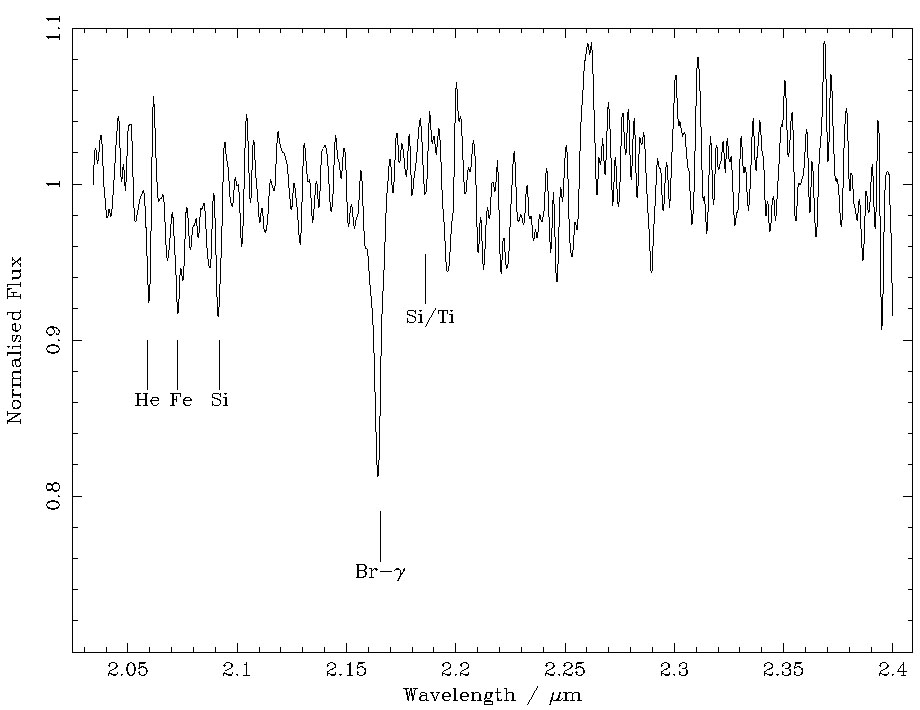
\includegraphics[width=5.0in]{j1655editedMasked}
\caption{%
The $K$--band spectrum of \groj, having been corrected for telluric
features with reference to an A0 star. The dominant Br-$\gamma$
feature is marked, together with several weaker features. }
\label{cha:AccretionDiskContamination:sec:Spectroscopy:subsec:CombiningTheSpectra:fig:j1655editedMasked}
\end{center}
\end{figure}
%%%%%%%%%%%%%%%%%%%%%%%%%%%%%%%%%%%%%%%%%%%%%%%%%%%%%%%%%%%%%%%%%%

The final spectrum was obtained by combining the two corrected target spectra, and smoothing the resultant spectrum, as we explained in \S~\ref{cha:InfraredDataReductionTechniques:sec:SpectroscopyData:subsec:CombiningTheSpectra}. Our spectrum of \groj\ is shown in Figure~%
\ref{cha:AccretionDiskContamination:sec:Spectroscopy:subsec:CombiningTheSpectra:fig:j1655editedMasked}%
. %

%%%%%%%%%%%%%%%%%%%%%%%%%%%%% Disk Contribution %%%%%%%%%%%%%%%%%%%%

\subsection{Determining the Disk Contribution}
\label{cha:AccretionDiskContamination:sec:Spectroscopy:subsec:DiskContribution}

%%%%%%%%%%%%%%%%%%%%%%%%%%%%% combinedSpectra %%%%%%%%%%%%%%%%%%%%
\begin{figure}[!htb]
\begin{center}
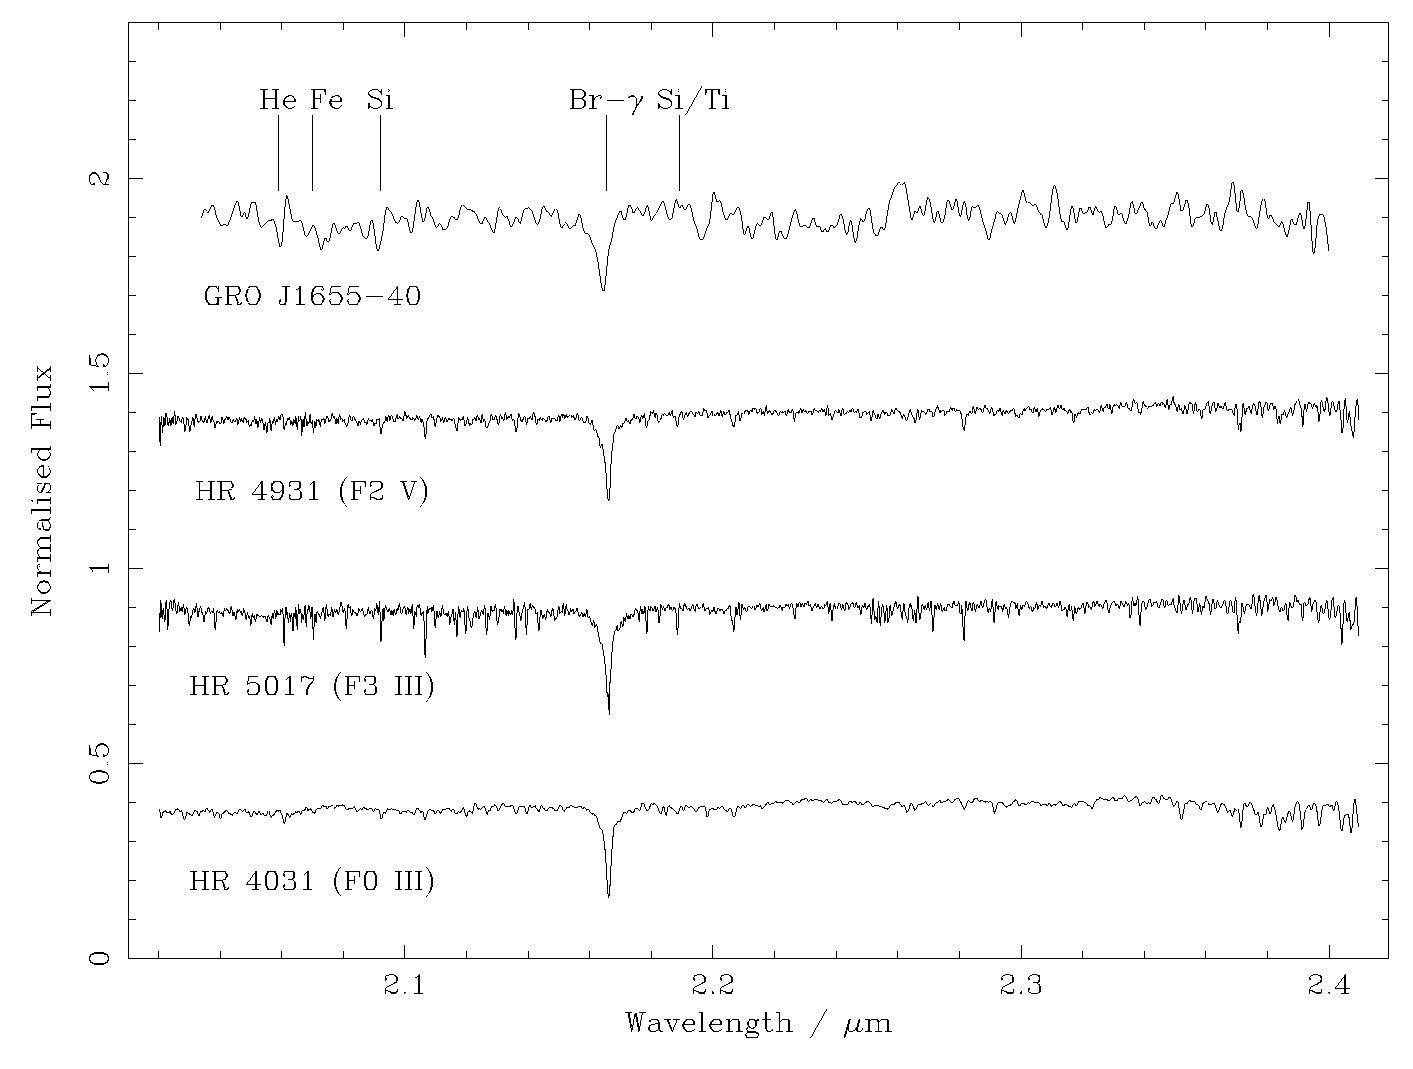
\includegraphics[width=5.0in]{combinedSpectra}
\caption{%
The $K$--band spectra of GRO J1655--40, HR 4031, HR 5017 and HR 4931, with the
spectral features of interest marked.}
\label{cha:AccretionDiskContamination:sec:Spectroscopy:subsec:DiskContribution:fig:combinedSpectra}
\end{center}
\end{figure}
%%%%%%%%%%%%%%%%%%%%%%%%%%%%%%%%%%%%%%%%%%%%%%%%%%%%%%%%%%%%%%%%%%


In order to determine the degree of accretion disk contamination in
\groj, we compared our spectrum of this system with spectra of
isolated stars of similar spectral type to the secondary in \groj. We
obtained these comparison spectra from the literature, and calculated
the equivalent width (see
\S~%
\vref{cha:InfraredDataReductionTechniques:sec:Spectroscopy:subsec:EquivalentWidth}%
) of the Br-$\gamma$ absorption feature in the target and comparison
spectra. If the Br-$\gamma$ feature in our spectrum of \groj\ was
significantly weaker than the corresponding features in the sample
spectra, this would imply that there was emission present in the $K$--band from the
disk. %

\vspace{\myparskip}

\begin{table}[htb]
\caption{Equivalent widths of Br-$\gamma$ feature}
\label{cha:AccretionDiskContamination:sec:Spectroscopy:subsec:AbsenceOfDiskContribution:tab:WallaceWidths}

\begin{minipage}{\linewidth}
\renewcommand{\thefootnote}{\thempfootnote}

\begin{center}
\begin{tabular}{|l|l|c||||l|l|c|}

\hline
Identifier & Spectral Type & $W_{\lambda}/$\AA & Identifier & Spectral
Type & $W_{\lambda}/$\AA \\\hline\hline\hline\hline
\groj\  & F5--G0 III--IV & $10\pm1$ & \mbox{HR 4931} & F2 V & $8\pm1$ \\\hline
\mbox{HR 7495} & F5 II--III & $7.0\pm0.5$ & \mbox{HR 6927} & F7 V & $4.0\pm0.5$ \\\hline
\mbox{HR 4031} & F0 III     & $8.5\pm0.5$ & \mbox{HR 6608} & G2 IIIb & $3.0\pm0.5$ \\\hline
\mbox{HR 5017} & F3 III     & $8\pm1$     & \mbox{HR 7373} & G8 IV & $3\pm1$ \\\hline
\mbox{HR 21}   & F2 IV      & $7\pm1$     & \mbox{HR 4375} & G0 V & $3\pm1$ \\\hline
\mbox{HR 8905} & F8 IV      & $4.5\pm0.5$ & \mbox{HR 483}  & G1.5 V & $3.5\pm0.5$ \\\hline
\mbox{HR 2943} & F5 IV-V    & $6.5\pm0.5$ & \mbox{HR 7504} & G3 V & $3.0\pm0.5$ \\\hline
\hline
\end{tabular}
\end{center}
\end{minipage}
\end{table}

The isolated stars with spectral types of F5--G0 III--IV (the spectral
type of \groj: see %
\citeNP{BeerPodsiadlowski:2001}%
) were chosen from the spectral atlas
of %
\citeN{WallaceHinkle:1997}%
. Figure~%
\vref{cha:AccretionDiskContamination:sec:Spectroscopy:subsec:DiskContribution:fig:combinedSpectra}%
\ displays three of the chosen spectra%
\footnote{%
\label{cha:AccretionDiskContamination:sec:Spectroscopy:subsec:DiskContribution:foot:wavenumber}%
The spectra were originally plotted with flux as a function of inverse wavenumber, but we converted them to $\mu$m for comparison with our spectrum. %
}%
, together with our spectrum of \groj. The equivalent widths of the Br-$\gamma$ absorption features in the telluric-corrected spectrum of \groj\ and the above stars were measured using \texttt{splot}. Table~%
\vref{cha:AccretionDiskContamination:sec:Spectroscopy:subsec:AbsenceOfDiskContribution:tab:WallaceWidths}%
\ lists these equivalent widths. %

\vspace{\myparskip}

As can be clearly seen, the equivalent width for \groj\ agrees well
with certain stars, namely \mbox{HR 4031}, \mbox{HR 5017} and \mbox{HR
4931}. This implies that the disk contributes little light to the
system in the $K$--band, and also that the spectral type of the secondary
star in \groj\ is within the range F5--F7 III--IV, which is consistent
with our initial range of F0--G2 III--IV, derived in \S~%
\vref{cha:lightcurve:sec:Photometry:subsec:DereddenedMagnitude}%
. %

\vspace{\myparskip}

\begin{table}[htb]
\caption{Equivalent widths of weaker features}
\label{cha:InfraredDataReductionTechniques:sec:Spectroscopy:subsec:AbsenceOfDiskContribution:tab:Weaker}

\begin{minipage}{\linewidth}
\renewcommand{\thefootnote}{\thempfootnote}

\begin{center}
\begin{tabular}{|l||||c|c|c|c|}

\hline
Identifier     & He        & Fe            & Si           & Si/Ti  \\\hline\hline\hline\hline
\groj\      & $1.1\pm0.2$     & $0.8\pm0.3$      & $1.1\pm0.2$     & $0.5\pm0.2$    \\\hline
HR 4031      & $0.6\pm0.1$     & $0.4\pm0.1$      & $0.3\pm0.1$     & $0.4\pm0.1$    \\\hline
HR 5017      & $0.2\pm0.1$     & $0.6\pm0.1$      & $0.4\pm0.1$     & $0.5\pm0.1$    \\\hline
HR 4931      & $0.4\pm0.2$     & $0.5\pm0.1$      & $0.3\pm0.1$     & $0.3\pm0.1$    \\\hline

\hline

\end{tabular}
\end{center}
\end{minipage}
\end{table}

As well as comparing the equivalent widths of the Br-$\gamma$ features
in our spectra and those of %
\citeN{WallaceHinkle:1997}%
, we also compared the equivalent widths of weaker features that we could identify in these
spectra. These were the He feature at
$\lambda=20\,590$\,\AA, the Fe line at $\lambda=20\,700$\,\AA, the Si
feature at $\lambda=21\,360$\,\AA\ and the combined Si/Ti absorption at
$\lambda=21\,890$\,\AA. The equivalent widths obtained are listed in
Table%
\vref{cha:InfraredDataReductionTechniques:sec:Spectroscopy:subsec:AbsenceOfDiskContribution:tab:Weaker}%
. %

\vspace{\myparskip}

Although the equivalent widths from the sample spectra are not in
complete agreement with our results, there is at least no evidence of
emission from the disk, as the absorption features in our spectrum are
stronger. We can therefore conclude that there is negligible disk
contamination in \groj\ during quiescence. We compared our results with those of Israelian~et~al.\ %
\citeyear{Israelian_et_al.:1999}%
, who found that the atmosphere of \groj\ was similar to that of a standard F6--F7 III--IV star, with an almost solar Fe abundance. They did find, however, an overabundance of $\alpha$--elements, such as Si and Ti. Our results support these conclusions. %

\vspace{\myparskip}

Hence, there is no evidence of emission from the disk, and we can conclude that there is negligible disk contamination in \groj\ during quiescence. %

%%%%%%%%%%%%%%%%%%%%%%%%%%%%% Radial velocity %%%%%%%%%%%%%%%%%%%%

\subsection{Calculating the Radial Velocity}
\label{cha:AccretionDiskContamination:sec:Spectroscopy:subsec:RadialVelocity}

As a check for consistency, we calculated the radial velocity of the
secondary star in \groj from the published spectroscopic ephemeris during the time of the observation, and compared
this theoretical value with that derived from our spectra of this
system. %

\vspace{\myparskip}

We first determined from the Universal Date and Time of
the observation of \groj\ and using the ephemeris of van~der~Hooft et~al.\ %
\citeyear{VanDerHooft_et_al.:1998}%
\ that the system was at phase 0.05. Using the values for $\gamma$ and
$K_2$ from %
\citeN{OroszBailyn:1997}%
, namely:
\begin{eqnarray}
\label{cha:AccretionDiskContamination:sec:Spectroscopy:subsec:RadialVelocity:eqn:values}
\gamma = -142.4\pm1.6\,\mathrm{km\,s}^{-1},\\
K_2 = 228.2\pm2.2\,\mathrm{km\,s}^{-1},
\end{eqnarray}
we determined that the radial velocity of the secondary at phase
0.05 should be $v_r = -142\pm2\,\mathrm{km}\,\mathrm{s}^{-1}$. %

\vspace{\myparskip}

From our telluric-corrected spectrum of \groj, we determined the
wavelength of the Br-$\gamma$ feature to be
$\lambda_{\mathrm{obs}}=21\,644.41$\,\AA. Using Equation~%
\vref{cha:InfraredDataReductionTechniques:sec:Spectroscopy:subsec:RadialVelocity:eqn:vr2}%
, we calculated that the corresponding radial velocity of the
secondary star is $v_r = -147\pm5\,\mathrm{km}\,\mathrm{s}^{-1}$. We
therefore conclude that the Doppler shift of the spectral features of
the secondary star due to its radial velocity are as expected. %

%%%%%%%%%%%%%%%%%%%%%%%%%%%%% Negligible Disk Contamination %%%%%%%%%%%%%%%%%%%%

\section{Negligible Disk Contamination!}
\label{cha:AccretionDiskContamination:sec:NegligibleDiskContamination}

Having confirmed that \groj\ was indeed in quiescence during our observations in 1998, with little contribution from the accretion disk to the total flux from the binary, we can have confidence in our derived value for the mass ratio, the inclination and most importantly the mass of the black hole. %

%%%%%%%%%%%%%%%%%%%%%%%%%%%%% End of Chapter %%%%%%%%%%%%%%%%%%%%
